\subsubsection{Tracking}
\label{subsec:03tracking}
Da die Detektion einen gewissen Rechenaufwand und somit Rechenzeit ben\"otigt, kann sie aufgrund den begrenzten Hardwareressourcen nicht regelm\"a{\ss}ig durchgef\"uhrt werden. Aus diesem Grund wird in der zweiten Phase der Personenverfolgung Tracking genutzt. \\
Tracking ist ein Vorgehen, um Objekte, in unserem Fall eine Person, in einer Folge von Bildern zu verfolgen. Der Vorteil von Tracking ist die rechensparsame Berechnung der n\"achsten Position eines Objekts, die unter gewissen Bedingungen sogar robuster als eine Detektion sein kann. Jedoch muss Tracking zu Beginn initialisiert werden, das durch die Bounding-Box der Detektion bereits gegeben ist. Zur Umsetzung des Trackings existieren verschiedene Ans\"atze, die einzelne Pixel, einen ganzen Bildteil oder Bewegungen im Bild nutzen. \\
Eine Auswahl an f\"unf Trackern wurden bereits in der OpenCV-Tracking API implementiert, sodass mehrere Tracker f\"ur die gegebene Anwendung getestet werden konnten. Die Tracker verwenden jeweils die interne Representation einer Bounding-Box und lernen abgesehen vom Median Flow einen Klassifizierer mithilfe von Online Learning\footnote{https://www.learnopencv.com/object-tracking-using-opencv-cpp-python/}. Als geeignetester Tracker stellte sich bei der Versuchsreihe der Median Flow heraus. Er bietet den besten Tradeoff zwischen Rechenzeit und Robustheit bei der Personenverfolgung. Die relativ langsamen und vorhersagbare Bewegung einer Person eignen sich gut f\"ur den gew\"ahlten Tracker. \\
Der Median Flow besteht aus zwei Hauptkomponenten. Im ersten Schritt wird die Bewegung ausgew\"ahlter Pixel mithilfe des Lucas-Kanade-Trackers berechnet und anschlie{\ss}end wird die berechnete Position durch den Forward/Backward-Error evaluiert. Die beiden Komponenten werden im Folgenden nochmal genauer beschrieben:
\paragraph{Lucas-Kanade-Tracker}
Der Lucas-Kanade-Tracker basiert auf dem Prinzip des Optischen Flusses. So kann in einer Bildfolge die neue Position eines Pixels mit folgendem Zusammenhang ausgedr\"uckt werden:
\begin{align}
I(x,y,t)=I(x+dx,y+dy,t+dt)
\end{align}
Hierbei beschreibt $I(x,y,t)$ die Intensit\"at eines Pixels an der Position $(x,y)$ zum Zeitpunkt $t$. Durch die Linearisierung mithilfe Taylorreihenentwicklung ergibt sich die Formel des Optischen Flusses zu
\begin{align}
I_{x}u+I_{y}v+I_{t} = 0 
\end{align}
mit 
\begin{align}
u=\frac{dx}{dt},\ v=\frac{dy}{dt},\ I_{x}=\frac{dI}{dx},\ I_{y}=\frac{dI}{dy},\ I_{t}=\frac{dI}{dt}.
\end{align}
Nun besteht die Aufgabe die Bewegeung $(u,v)$ zu bestimmen. Dies wird mithilfe der Erweiterung der Gleichung unter Einbeziehung der benachbarten Pixel in einem $3x3$ Fenster erm\"oglicht:
\begin{align}
\begin{pmatrix}
I_{x}(p_{1}) & I_{y}(p_{1}) \\ 
... & ...\\ 
I_{x}(p_{9}) & I_{y}(p_{9})
\end{pmatrix} 
\begin{pmatrix}
u\\ 
v
\end{pmatrix}+
\begin{pmatrix}
I_{t}(p_{1})\\ 
...\\ 
I_{t}(p_{9})
\end{pmatrix} = 0
\end{align}
Die \"uberbestimmte Formel beinhaltet die 9 Pixel $p_{1}...p_{9}$ aus dem $3x3$ Fenster und kann mithilfe der Methode der kleinsten Quadrate gel\"ost. Als Ergebnis erh\"alt man die Bewegung eines Pixels, die die Verfolgung über eine Folge von Bildern erm\"oglicht.
\paragraph{Forward/Backward Error}
Mithilfe des Lucas-Kanade-Trackers wird ein Pixels �ber eine Bilderfolge von $k$ Bildern verfolgt und so eine Trajektorie $T^{k}_{f}=(x_{t},x_{t+1},...,x_{t+k})$ bestimmt. Hierbei steht $f$ f\"ur $forward$ und beschreibt die Forw\"artstrajektorie. Das Ziel ist nun diese Trajektorie zu validieren. Hierf�r beginnen wir bei dem $x_{t+k}$ und verfolgen diesen Pixel r\"uckw\"arts �ber die gegebene Folge von $k$ Bildern. So wird eine zweite Trajektorie $T^{k}_{b}=(\hat{x}_{t},\hat{x}_{t+1},...,\hat{x}_{t+k})$ bestimmt, die mit der ersten verglichen wird. Um die Berechnung simpel zu halten, wird die euklidische Distanz zwischen Start und Endpunkt der jeweiligen Trajektorie gew�hlt:
\begin{align}
distance(T^{k}_{f},T^{k}_{b})= \left \| x_{t} - \hat{x}_{t} \right \|
\end{align} 
In Abbildung \ref{fig:ForBackError} wird das Vorgehen zur Bestimmung des Forward/Backward Errors nochmals veranschaulicht. \\
\begin{figure}[h]
	\centering
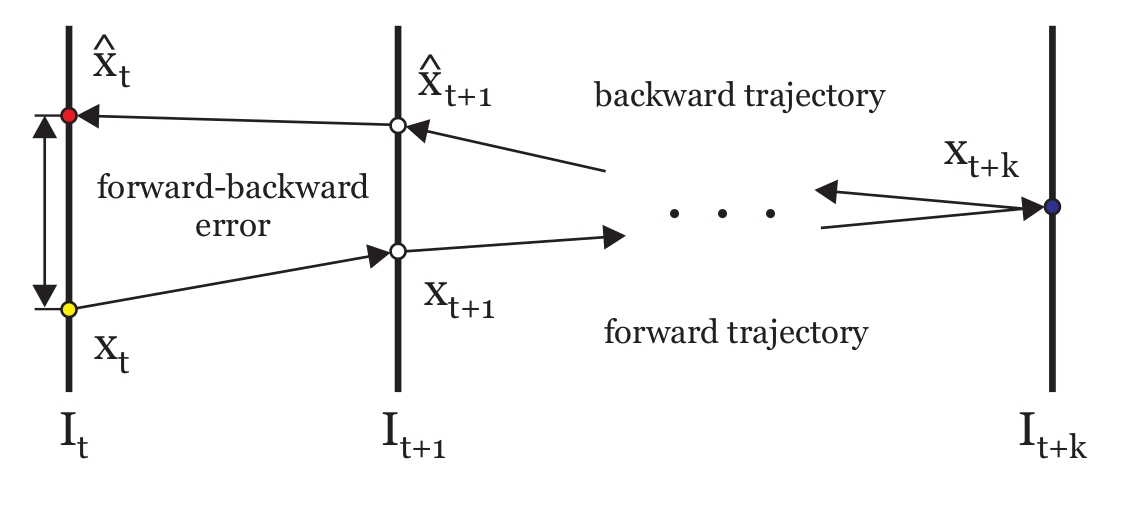
\includegraphics[width=0.6\textwidth,trim=2.4cm 0cm 0cm 1cm,clip]{pics/ForwardBackwardE.jpg}
	\caption{Das Vorgehen zur Berechnung des Forward/Backward Errors. (Quelle)}
	\label{fig:ForBackError}
\end{figure} \\

Die beschriebene Methode zur Validierung wird in der Implementierung des Median Flow zwei mal angewendet. Zu Beginn wird sie zur Auswahl der Featurpunkte aus dem Detektionfenster, die mit dem Ansatz von Lucas und Kanade getrackt werden, genutzt. So werden die Pixel, die einen hohen Forward/Backward Error aufweisen, verworfen und die signifikanten f�r Tracking geeignete Feature behalten. Weiterhin wird der Fehler zur Validierung des gesamten Trackingergebnisses genutzt und kann so ein fehlerhaftes Tracking erkennen und abrechen.